
%(BEGIN_QUESTION)
% Copyright 2006, Tony R. Kuphaldt, released under the Creative Commons Attribution License (v 1.0)
% This means you may do almost anything with this work of mine, so long as you give me proper credit

Beregn kraften som genereres i det store stempelet (areal = 40 in$^{2}$), gitt en kraft på 25 pund som virker på det lille stempelet (areal = 10 in$^{2}$).  Beregn også trykket der de to trykkmålerne er plassert, og forklar hvordan det hydrostatiske trykket fra vannsolens vertikale høyde på 20 fot virker inn på denne kraftberegningen.

$$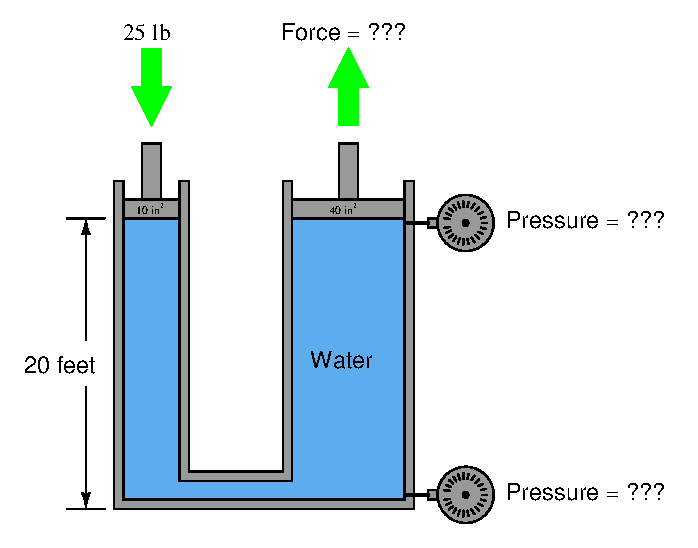
\includegraphics[width=15.5cm]{i00159x01.eps}$$

Representerer forskjellen i trykk mellom de to målepunktene et brudd på Pascals prinsipp?  Hvorfor eller hvorfor ikke?

\underbar{file i00159}
%(END_QUESTION)





%(BEGIN_ANSWER)

Kraft i stort stempel = 100 pund.

\vskip 10pt

Den øvre trykkmåleren vil vise 2.5 PSI, og den nedre trykkmåleren vil vise 11.17 PSI.

\vskip 10pt

Pascals prinsipp kan uttrykkes presist slik:

\vskip 10pt {\narrower \noindent \baselineskip5pt
``Trykk som pålegges en innestengt væske øker trykket i hele væskevolumet med samme beløp''
\par} \vskip 10pt

Matematisk kan Pascals prinsipp skrives slik:

$$\Delta P_1 = \Delta P_2$$

Det ville være feil å anta at trykket i hele et innestengt væskevolum er det samme (dvs. $\Delta P_1 = \Delta P_2$), fordi det ville utelukke hydrostatisk trykk som avhenger av høyde.  Det er mer korrekt å formulere Pascals prinsipp i form av \textit{trykkøkning}.

%(END_ANSWER)





%(BEGIN_NOTES)


%INDEX% Physics, fluids: pressure, force, and area
%INDEX% Physics, static fluids: Pascal's Principle

%(END_NOTES)

